\documentclass[12pt]{article}
\usepackage[margin=2.5cm]{geometry}
\usepackage{enumerate}
\usepackage{amsfonts}
\usepackage{amsmath}
\usepackage{fancyhdr}
\usepackage{amsmath}
\usepackage{amssymb}
\usepackage{amsthm}
\usepackage{mdframed}
\usepackage{graphicx}
\usepackage{subcaption}
\usepackage{adjustbox}
\usepackage{listings}
\usepackage{xcolor}
\usepackage{courier}
\usepackage[utf]{kotex}
\usepackage{hyperref}

\definecolor{codegreen}{rgb}{0,0.6,0}
\definecolor{codegray}{rgb}{0.5,0.5,0.5}
\definecolor{codepurple}{rgb}{0.58,0,0.82}
\definecolor{backcolour}{rgb}{0.95,0.95,0.92}

\lstdefinestyle{mystyle}{
    backgroundcolor=\color{backcolour},
    commentstyle=\color{codegreen},
    keywordstyle=\color{magenta},
    numberstyle=\tiny\color{codegray},
    stringstyle=\color{codepurple},
    basicstyle=\ttfamily\footnotesize,
    breakatwhitespace=false,
    breaklines=true,
    captionpos=b,
    keepspaces=true,
    numbers=left,
    numbersep=5pt,
    showspaces=false,
    showstringspaces=false,
    showtabs=false,
    tabsize=1
}

\lstset{style=mystyle}

\pagestyle{fancy}
\renewcommand{\headrulewidth}{0.4pt}
\lhead{CSC 369}
\rhead{Midterm 1 Solution}

\begin{document}
\title{CSC 369 Midterm 1 Solution}

\bigskip

\begin{enumerate}[1.]
    \item

    \begin{enumerate}[a)]
        \item Trap instruction is run in user mode, and privileged operation is
        run in kernel mode
        \bigskip

        \underline{\textbf{Notes}}

        \begin{itemize}
            \item \textbf{Previliged Instructions}

            \begin{itemize}
                \item Is the instruction that can run only in \textbf{kernel mode}
                \item Attempt at execution in \textbf{user mode} $\to$ treated as an illegal operation \& will not run.
            \end{itemize}

            \item \textbf{Trap}

            \begin{itemize}
                \item Is a special hardware instruction
                \item Is a software generated interrupt $^{[4]}$
                \item Is a type of synchronous interrupt $^{[1]}$
                \item Is caused by an exceptional condition $^{[1]}$

                \begin{enumerate}[1.]
                    \item Division by zero $^{[1]}$
                    \item Invalid memory access (segmentation fault) $^{[1]}$
                    \item Previleged instruction by \textbf{user mode} code $^{[2]}$
                \end{enumerate}
                \item Usually results in a switch to \textbf{kernel mode} $\to$ Operating system performs action $\to$
                Returns control to oroginal process
            \end{itemize}

            \item \textbf{Trap Instruction}

            \begin{itemize}
                \item Is executed when a user wants to invoke a service from the operating system (i.e. reading hard drive)
                in \textbf{user mode}
                \item Raise (the processor) privilege level to kernel mode
            \end{itemize}

            \item \textbf{User Mode}

            \begin{itemize}
                \item Is restricted
                \item Executing code has no ability to \textit{directly} access
                hardware or reference memory $^{[3]}$
                \item Crashes are always recoverable $^{[3]}$
                \item Is where most of the code on our computer / applications are executed $^{[3]}$
            \end{itemize}

            \item \textbf{Kernel Mode}
            \begin{itemize}
                \item Is previleged (non-restricted)
                \item Executing code has complete and unrestricted access to the underlying hardware $^{[3]}$
                \item Is generally reserved for the lowest-level, most trusted functions of the operating
                system $^{[3]}$
                \item Is fatal to crash; it will halt the entire PC (i.e the blue screen of death) $^{[3]}$
            \end{itemize}
        \end{itemize}

        \bigskip

        \underline{\textbf{References}}

        \begin{enumerate}[1)]
            \item Wikipedia, Trap (computing), \href{https://en.wikipedia.org/wiki/Trap_(computing)#:~:text=In%20computing%20and%20operating%20systems,zero%2C%20invalid%20memory%20access).}{link}
            \item University of Utah, CS5460: Operating Systems Lecture 3 - OS Organization, \href{https://my.eng.utah.edu/~cs5460/slides/Lecture03.pdf}{link}
            \item Coding Horror, Understanding User and Kernel Mode, \href{https://blog.codinghorror.com/understanding-user-and-kernel-mode/}{link}
            \item ETH Zurich, Programming in Systems, \href{link}{link}
        \end{enumerate}

        \item

        No. Lock uses a variable with binary states 0 (acquired) and 1 (available), where as
        semaphore uses counter variable that can have value greater than 1 to
        keep track of the amount of resource remaining.

        \bigskip

        \underline{\textbf{Notes}}

        \begin{itemize}
            \item \textbf{Locks}

            \begin{itemize}
                \item Is a variable with two boolean states

                \begin{itemize}
                    \item 1 - (available/unlock/free)
                    \item 0 - (acquired/locked/held)
                \end{itemize}

                \item Has two operations

                \begin{enumerate}[1.]
                    \item \texttt{acquire()}

                    \bigskip

                    \begin{center}
                    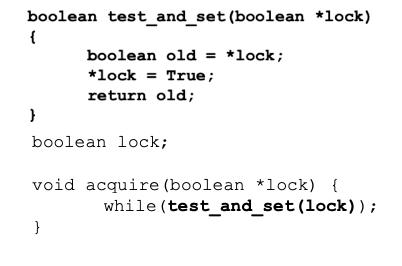
\includegraphics[width=0.7\linewidth]{images/midterm_1_solution_4.png}
                    \end{center}

                    \bigskip

                    \item \texttt{release()}

                    \bigskip

                    \begin{center}
                    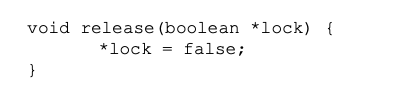
\includegraphics[width=0.7\linewidth]{images/midterm_1_solution_5.png}
                    \end{center}

                    \bigskip
                \end{enumerate}
                \item Is put around critical section to ensure critical section executes
                as if it's a single atomic instruction

                \begin{center}
                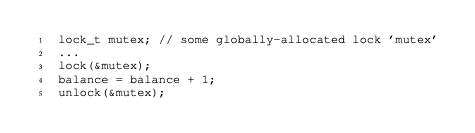
\includegraphics[width=\linewidth]{images/midterm_1_solution_1.png}
                \end{center}
                \item Can only be released by the thread that acquired it
                \item Is used to protect shared resource (e.g. from race condition in files and data structure) $^{[2]}$
            \end{itemize}

            \item \textbf{Semaphore}

            \begin{itemize}
                \item Is an abstract data types suitable for synchronization problems $^{[2]}$
                \item Has variable \texttt{count} that allows arbitrary resource count $^{[1]}$
                \item Has two atomic operations

                \begin{enumerate}[1.]
                    \item (\texttt{wait/P/decrement}) - block until \texttt{count $>$ 0} then decrement variable

                    \begin{center}
                    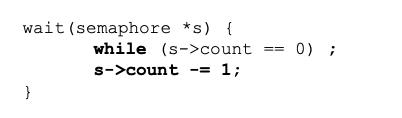
\includegraphics[width=0.7\linewidth]{images/midterm_1_solution_2.png}
                    \end{center}

                    \item (\texttt{signal/V/increment}) - increment \texttt{count}, unblock a waiting thread

                    \begin{center}
                    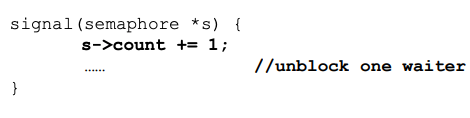
\includegraphics[width=0.7\linewidth]{images/midterm_1_solution_3.png}
                    \end{center}
                \end{enumerate}

                \item Can be signaled by any thread $^{[2]}$
            \end{itemize}
        \end{itemize}

        \bigskip

        \underline{\textbf{References}}

        \begin{enumerate}[1)]
            \item Wikipedia, Semaphore (programming), \href{https://en.wikipedia.org/wiki/Semaphore_(programming)}{link}
            \item Stack Overflow, Difference between binary semaphore and mutex, \href{https://stackoverflow.com/questions/62814/difference-between-binary-semaphore-and-mutex}{link}
        \end{enumerate}

        \item

        If both access are read, then concurrency error will not occur.

        \bigskip

        \underline{\textbf{Notes}}

        \begin{itemize}
            \item What is concurrency error? Where and when does it occur?

            \item \textbf{Concurrency}

            \begin{itemize}
                \item Is the ability of different parts or units of a program, algorithm,
                or problem to be \underline{executed out of order}, \underline{without affecting the final
                outcome}. $^{[1]}$
            \end{itemize}

            \item \textbf{Concurrency Error}

            \begin{itemize}
                \item Two types of concurrency errors $^{[3]}$

                \begin{enumerate}[1.]
                    \item \textbf{Deadlock:} A situation wherein two or more processes
                    are never able to proceed because each is waiting for the others
                    to do something

                    \bigskip

                    Key: Circular wait

                    \bigskip

                    \item \textbf{Race Condition:} a timing dependent error
                    involving shared state

                    \begin{itemize}
                        \item \textbf{Data Race:} Concurrent accesses to a shared variable
                        and at least one access is a write
                        \item \textbf{Atomicity Bugs:} Code does not enforce the atomicity
                        programmers intended for a group of memory access
                        \item \textbf{Order Bugs:} Code does not enforce the order programmers
                        intended for a group of memory access
                    \end{itemize}
                \end{enumerate}
            \end{itemize}

            \item \textbf{Thread}

            \begin{itemize}
                \item Is the smallest sequence of programmed instructions that can be managed independently
                by a schdeduler $^{[2]}$

                \begin{center}
                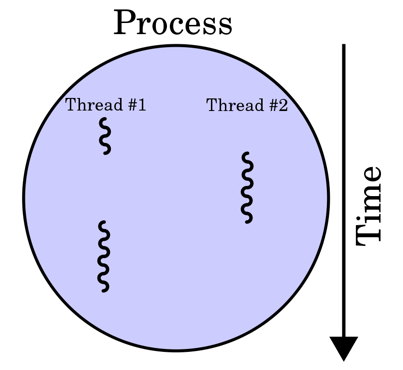
\includegraphics[width=0.4\linewidth]{images/midterm_1_solution_6.png}
                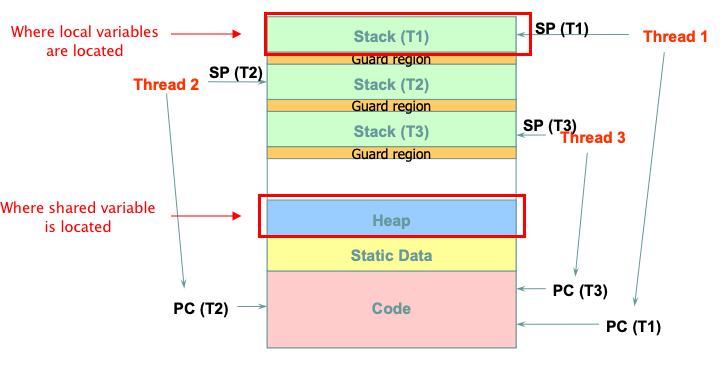
\includegraphics[width=\linewidth]{images/midterm_1_solution_7.png}
                \end{center}

                \item A thread is bound to a single process
                \item A process can have multiple threads
            \end{itemize}
        \end{itemize}

        \bigskip

        \underline{\textbf{References}}

        \begin{enumerate}[1)]
            \item Wikipedia, Concurrency (computer science), \href{https://en.wikipedia.org/wiki/Concurrency_(computer_science)}{link}
            \item Wikipedia, Thread, \href{https://en.wikipedia.org/wiki/Thread_(computing)#:~:text=In%20computer%20science%2C%20a%20thread,part%20of%20the%20operating%20system.}{link}
            \item Columbia University, Concurrency Errors, \href{https://www.cs.columbia.edu/~junfeng/13fa-w4118/lectures/l11-concurrency-error.pdf}{link}
        \end{enumerate}


        \item

        \bigskip

        No, limited execution limits what a process can do without OS assistance
        by restricting access to hardwares, setting up interrupt timer, and trap handlers.

        \bigskip

        \underline{\textbf{Notes}}

        \begin{itemize}
            \item \textbf{Virtualization of CPU}

            \begin{itemize}
                \item
            \end{itemize}
            \item \textbf{Limited Direct Execution}

            \begin{itemize}
                \item Idea: Just run the program you want to run on the CPU,
                but first make sure to set up the hardware so as to limit what
                process can do without OS assistance
                \item baby proofs the CPU by

                \bigskip

                \begin{enumerate}[1.]
                    \item Setting up trap handlers
                    \item Starts an interrupt timer
                    \item Run processes in a restricted mode
                \end{enumerate}

                \bigskip

                \underline{\textbf{Example}}

                \bigskip

                Baby proofing a room:

                \bigskip

                \begin{itemize}
                    \item Locking cabinets containing dangerous stuff and covering electrical sockets.
                    \item When room is readied, let your baby roam free in knowledge that all the dangerous
                    aspect of the room is restricted
                \end{itemize}
            \end{itemize}

            \item \textbf{Trap Handlers}

            \begin{itemize}
                \item Is instruction that tells the hardware what to run when certain exceptions occur

                \bigskip

                \underline{\textbf{Example}}

                \bigskip

                What code to run when

                \begin{enumerate}[1.]
                    \item Hard disk interrupt occurs
                    \item Keyboard interrupt occrs
                    \item Program makes a system call?
                \end{enumerate}

            \end{itemize}

            \item \textbf{Timer Interrupt}

            \begin{itemize}
                \item Is a hardware mechanism that ensures the user program does not run forever
                \item Is emitted at regular intervals by a timer chip $^{[1]}$
            \end{itemize}
        \end{itemize}

        \bigskip

        \underline{\textbf{References}}

        \begin{enumerate}[1)]
            \item Wikibooks, Operating System Design/Processes/Interrupt, \href{https://en.wikibooks.org/wiki/Operating_System_Design/Processes/Interrupt#:~:text=Perhaps%20the%20most%20important%20interrupt,processor%20executing%20a%20specific%20instruction.}{link}
        \end{enumerate}

        \item

        \bigskip

        No, alhtough data blocks are fragmented, it doesn't suffer from external
        fragmentation because indexed file system has pointers in inodes that
        points to each data block.

        \bigskip

        \underline{\textbf{Notes}}

        \begin{itemize}

            \item \textbf{Index-based File System}

            \begin{center}

            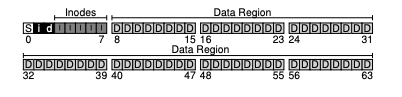
\includegraphics[width=\linewidth]{images/midterm_1_solution_8.png}
            \end{center}

            \begin{itemize}
                \item Has following parts

                \begin{itemize}
                    \item Superblock
                    \item Inode Bitmap
                    \item Data Bitmap
                    \item Inodes
                    \item Data Region
                \end{itemize}

                \item Each block in file system is 4KB
                \item Uses a large amount of metadata per file (especially for large files)
            \end{itemize}

            \item \textbf{Superblock}

            \begin{center}
            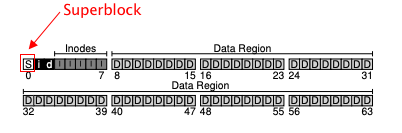
\includegraphics[width=\linewidth]{images/midterm_1_solution_9.png}
            \end{center}

            \begin{itemize}
                \item contains information about the file system, including

                \begin{enumerate}[1.]
                    \item the number of inodes and data blocks in a particular file system
                    \item the magic number of some kind to identify the file system type (e.g NFS, FFS, VSFS)
                \end{enumerate}

                \item The OS reads superblock \underline{first} to initialize various parameters,
                and then attach volume to the file-system tree
            \end{itemize}

            \item \textbf{Bitmap}

            \begin{center}
            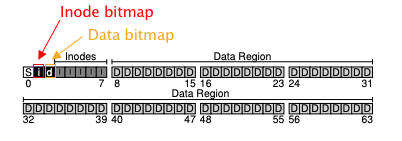
\includegraphics[width=\linewidth]{images/midterm_1_solution_10.png}
            \end{center}

            \begin{itemize}
                \item Tracks whether inode or data blocks are free or allocated
                \item Is a simple and popuar structure
                \item Uses each bit
                \begin{itemize}
                    \item \texttt{0} means free
                    \item \texttt{1} means in use
                \end{itemize}

                \item \textbf{Data Bitmap} is bitmap for data region
                \item \textbf{Inode Bitmap} is bitmap for inode region
            \end{itemize}

            \item \textbf{Inode}

            \begin{center}
            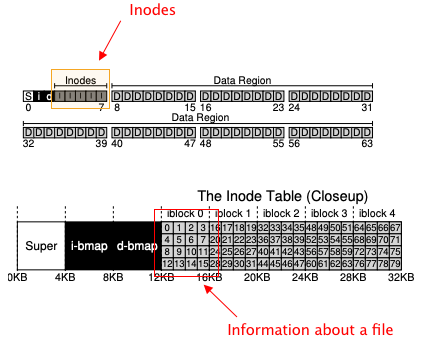
\includegraphics[width=\linewidth]{images/midterm_1_solution_12.png}
            \end{center}

            \begin{itemize}
                \item Is a short form for \textbf{index node}
                \item Contains disk block location of the object's data $^{[1]}$
                \item Contains all the information you need about a file (i.e. metadata)

                \begin{itemize}
                    \item File Type
                    \begin{itemize}
                        \item e.g. regular file, directory, etc
                    \end{itemize}
                    \item Size
                    \item Number of blocks allocated to it
                    \item Protection information
                    \begin{itemize}
                        \item such as who owns the file, as well as who can access it
                    \end{itemize}
                    \item Time information
                    \begin{itemize}
                        \item e.g. When file was created, modified, or last accessed
                    \end{itemize}
                    \item Location of data blocks reside on disk
                \end{itemize}
            \end{itemize}

            \item \textbf{Data Region}

            \begin{center}
            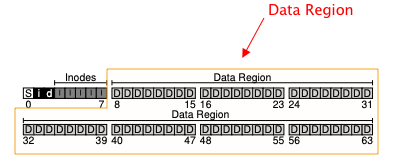
\includegraphics[width=\linewidth]{images/midterm_1_solution_11.png}
            \end{center}

            \begin{itemize}
                \item Is the region of disk we use for user data
            \end{itemize}

            \item \textbf{Multi-Level Index}

            \begin{center}
            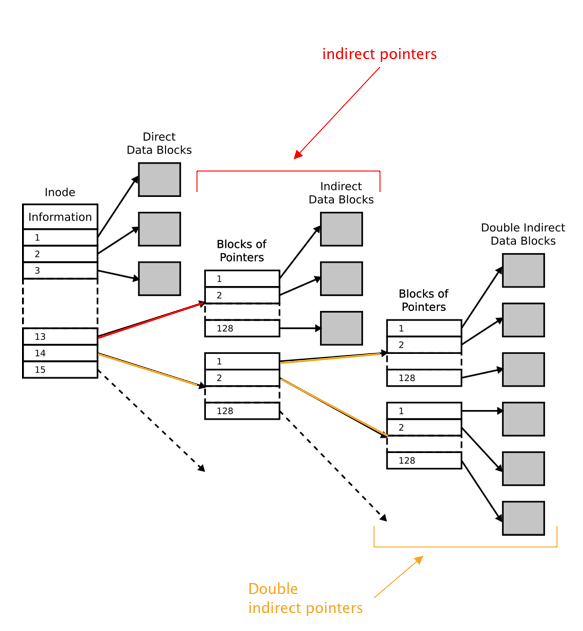
\includegraphics[width=\linewidth]{images/midterm_1_solution_13.png}
            \end{center}

            \begin{itemize}
                \item Is for supporting bigger files
                \item Uses \textbf{indirect pointer} in inode that points to more pointers
                \item Uses \textbf{double indirect pointer} for even larger files

                \begin{itemize}
                    \item is a pointer in inode that points to a block that contains
                    pointers to indirect blocks
                \end{itemize}
            \end{itemize}

            \item \textbf{External Fragmentation}

            \begin{itemize}
                \item Is various free holes that are generated in either your
                memory or disk space. $^{[2]}$
                \item Are available for allocation, but may be too small to be of
                any use $^{[2]}$
            \end{itemize}

            \item \textbf{Internal Fragmentation}

            \begin{itemize}
                \item Is wasted space within each allocated block $^{[2]}$
                \item Occurs when more computer memory is allocated than is needed
            \end{itemize}
        \end{itemize}

        \bigskip

        \underline{\textbf{References}}

        \begin{enumerate}[1)]
            \item Wikipedia: inode, \href{https://en.wikipedia.org/wiki/Inode}{link}
            \item Washington University, Explain the difference between external fragmentation
            and internal fragmentation, \href{https://courses.cs.washington.edu/courses/cse451/00sp/misc/quiz2sol.txt}{link}
            \item Wikipedia, Inode pointer structure, \href{https://en.wikipedia.org/wiki/Inode_pointer_structure}{link}
        \end{enumerate}

        \item

        \bigskip

        No, extent-based file system requires less disk block access, because unlike
        index-based file system (which consumes disk space for many indirect pointers
        in addition to data blocks for large files), extent-based file system only
        requires one pointer plus contiguous data blocks.

        \bigskip

        \underline{\textbf{Notes}}

        \begin{itemize}
            \item \textbf{Extent Based File System}

            \begin{center}
            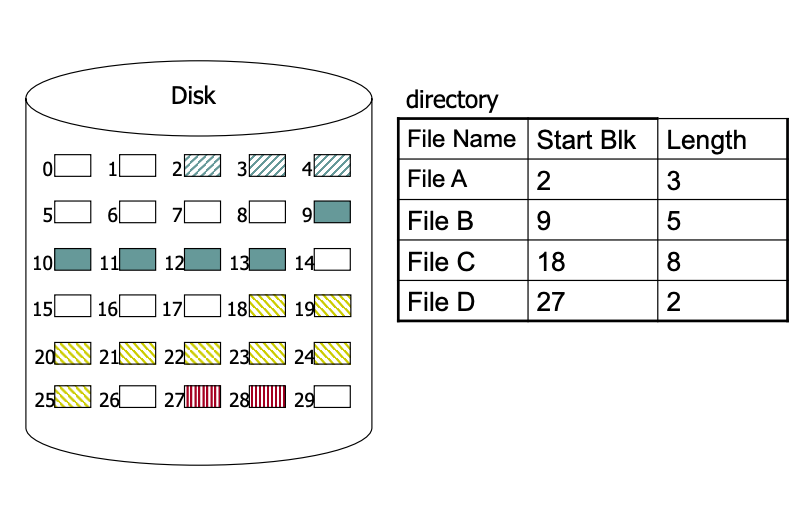
\includegraphics[width=\linewidth]{images/midterm_1_solution_14.png}
            \end{center}

            \begin{itemize}
                \item Is simply a disk pointer plus a length (in blocks)
                \begin{itemize}
                    \item Together, is called \textbf{extent}
                \end{itemize}
                \item Often allows more than one extent
                \begin{itemize}
                    \item resolve problem of finding continuous free blocks
                \end{itemize}
                \item Is less flexible but more compact
                \item Works well when there is enough free space on the disk and
                files can be laid out contiguously
            \end{itemize}

            \bigskip

            \underline{\textbf{Example}}

            \bigskip

            Linux's ext4 file system
        \end{itemize}
    \end{enumerate}

    \item

    \bigskip

    \begin{enumerate}[a)]

        \item

        \begin{enumerate}[1)]
            \item Process State
            \item Process Number
            \item CPU scheduling information / Process Priority
        \end{enumerate}

        \bigskip

        \underline{\textbf{Notes}}

        \begin{itemize}
            \item \textbf{Fields}

            \begin{itemize}
                \item Is the members in a structure

                \bigskip

                \begin{center}
                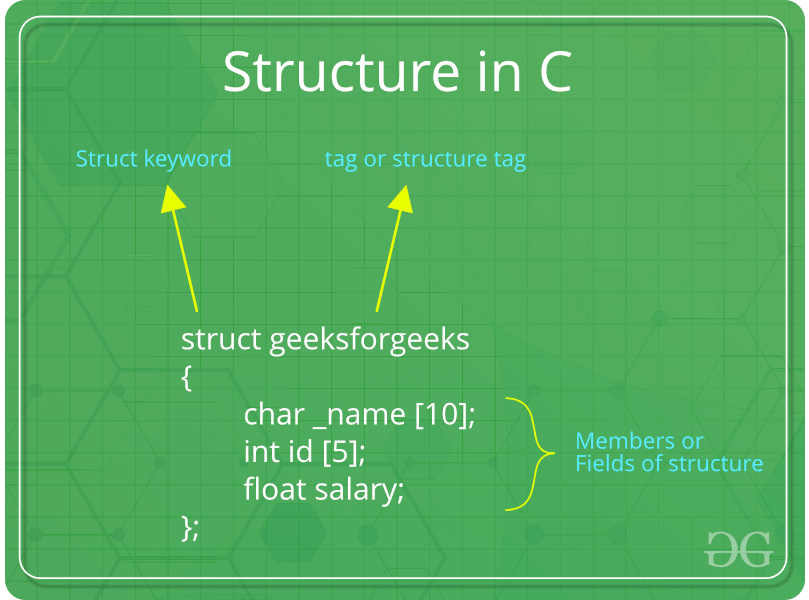
\includegraphics[width=0.6\linewidth]{images/midterm_1_solution_15.png}
                \end{center}
            \end{itemize}

            \item \textbf{Process List}

            \begin{itemize}
                \item Is a data structure in kernel or OS
                \item Contains information about all the processes running in the system
            \end{itemize}

            \item \textbf{Process Control Block}

            \begin{itemize}
                \item Is a data structure in kernel or OS
                \item Contains all information about a process
                \item Is where the OS keeps all of a process' hardware execution state
                \item Generally includes

                \begin{enumerate}[1.]
                    \item Process state (ready, running, blocked)
                    \item Process number
                    \item Program counter: address of the next instruction
                    \item CPU Registers: is saved at an interrupt
                    \item CPU scheduling information: process priority
                    \item Memory management info: page tables
                    \item I/O status information: list of open files
                \end{enumerate}
            \end{itemize}
        \end{itemize}

        \item

        Context switch switches from the current process to a different one.
        To achieve this, all resource information about process needs to be saved,
        including:

        \begin{itemize}
            \item Process Number
            \item Process State
            \item Process Counter,
            \item CPU Registers
            \item Memory management info
            \item I/O status Information
        \end{itemize}

        \underline{\textbf{Notes}}

        \begin{itemize}
            \item I am reading that process needs to save resource information
            before context switch. I need to verify with professor regarding this information.
            \item \textbf{Context Switch}

            \begin{itemize}
                \item is the process of storing the state of a process or thread,
                so it can be restored and resume execution at a later point $^{[1]}$
                \item happens during a timer interrupt or system call
                \item process context switch needs to save the following $^{[2]}$

                \begin{itemize}
                    \item Process Number
                    \item Process State
                    \item Process Counter,
                    \item CPU Registers
                    \item Memory management info
                    \item I/O status Information
                \end{itemize}

                \item thread context switch needs to save the following

                \begin{itemize}
                    \item Process Counter,
                    \item CPU Registers
                \end{itemize}

                \item May hinder performance
            \end{itemize}
        \end{itemize}

        \bigskip

        \underline{\textbf{References}}

        \begin{enumerate}[1)]
            \item Wikipedia: Context switch, \href{https://en.wikipedia.org/wiki/Context_switch}{link}
            \item University of Washington, CSE 451, Spring 2000 Solutions to Homework 2, \href{https://courses.cs.washington.edu/courses/cse451/00sp/homeworks/hw2soln.txt}{link}
        \end{enumerate}

        \item

        \bigskip

        One concrete example is CPU virtualization.

        \bigskip

        In this case, CPU is virtualized, and OS achieves CPU virtualization by

        \bigskip

        \begin{enumerate}[1)]
            \item Limiting the process can do without OS assistance by setting up trap handler and starting an interrupt timer
            \item Intervening at key points in time to perform privileged operations and
            switch out processes/operations that monopolized the CPU too long
        \end{enumerate}

        \bigskip

        \underline{\textbf{Notes}}

        \begin{itemize}
            \item \textbf{Virtualization}

            \begin{itemize}
                \item is an act of creating an illusion that there are as many hardware resource as each program needs.
            \end{itemize}

            \item \textbf{Virtualizing CPU}

            \begin{itemize}
                \item Turns a single CPU into a seemingly infinite number of CPUS, and
                allows many programs to seemingly run at once
                \item To implement CPU virtualization, the OS needs low-level machinery
                called \textbf{mechanism} and high level intelligence called \textbf{policies}
                \item Steps

                \begin{enumerate}[1.]
                    \item Involve OS to setup hardware hardwre to limit what the process can do without OS assistance
                    (\textbf{Limited Direct Execution})

                    \bigskip

                    This is done so by

                    \bigskip

                    \begin{enumerate}[1.]
                        \item Setting up trap handler
                        \item Starting an interrupt timer (so process won't last forever)
                    \end{enumerate}
                    \item Involve OS to intervene at key points to perform previleged operations
                    or switch out operations when they have monopolized the CPU too long
                \end{enumerate}
                \bigskip
            \end{itemize}

            \item \textbf{Limited direct execution}

            \begin{itemize}
                \item Is a mechanism of CPU virtualization
                \item Baby proofs the CPU by setting up hardwre to limit what the process can do without OS assistance
                \item Runs program in CPU once baby proofed
                \item Does so by
                \begin{itemize}
                    \item Setting up trap handler
                    \item Starting an interrupt timer (so process won't last forever)
                \end{itemize}
            \end{itemize}

            \item \textbf{Scheduling policies}

            \begin{itemize}
                \item Are series of polices of CPU virtualization

                \begin{itemize}
                    \item \textbf{First In First Out}
                    \item \textbf{Shortest Job First}
                    \item \textbf{Shortest Time-to-completion First}
                    \item \textbf{Round Robin}
                    \item \textbf{Multi-level Feedback Queue}
                \end{itemize}
            \end{itemize}

            \item \textbf{Virtualizing Memory}
            \begin{itemize}
                \item Basic Idea: For the most part, let the program run directly on the hardware;
                however, at certain key points in time (e.g. system call, timer interrupt), arrange
                so that the OS gets involved and make sure the 'Right' thing happens.
                \item Like CPU, many programs are sharing the memory at the same time
                \item Like CPU, the goal is to create an illusion that it has its own code and data
                \item Like CPU, the memory also needs low-level machinery called \textbf{mechanism},
                and high level intelligence called \textbf{policies}
                \item Steps

                \begin{enumerate}[1.]
                    \item Use \textbf{address translation} to transform each memory access,
                    changing \textbf{virtual address} provided by instruction to \textbf{physical address}
                    \begin{itemize}
                        \item Memory access includes instruction fetch, load, or store
                        \item Is done using hardware
                    \end{itemize}
                    \item Invove OS at key points to \textbf{manage memory}

                    \bigskip

                    Memory management includes

                    \bigskip

                    \begin{enumerate}[1.]
                        \item Setting up hardware so correct translations take place
                        \item Keeping track of which locations are free and which are in use
                        \item Judiciously intervening to maintain control over how memory is used
                    \end{enumerate}

                    \bigskip
                \end{enumerate}
            \end{itemize}

            \item \textbf{Address Translation}

            \begin{itemize}
                \item Is also called \textbf{hardware-based address translation}
                \item Is a mechanism of memory virtualization
                \item Is the technique of transforming virtual address to physical address
            \end{itemize}

            % \item \textbf{Dynamic (Hardware-based) Relocation}

            % \begin{itemize}
            %     \item Is a type of address translation
            %     \item Occured in 1950's
            %     \item Is also referred as \textbf{base and bounds}
            %     \item Need \textbf{base register} and the \textbf{bounds}

            %     \begin{itemize}
            %         \item \textbf{base register} transforms virtual address to physical address
            %         \item \textbf{bound} ensures addresses are within confines of the address space
            %     \end{itemize}
            %     \item Steps

            %     \begin{enumerate}[1.]
            %         \item Write and compile program as if it is loaded at address zero
            %         \item Allow OS to decide where in physical memory it should be loaded
            %         and set base register to that value

            %         \bigskip

            %         \texttt{physical address = virtual address + base}
            %     \end{enumerate}
            % \end{itemize}
        \end{itemize}


    \end{enumerate}

    \bigskip

    \item

    \texttt{a)}, \texttt{b)} and \texttt{c)} are true

    \bigskip

    \underline{\textbf{Notes}}

    \begin{itemize}
        \item I need clarification from professor on the meaning behind `Mutex is held?'
    \end{itemize}

    \bigskip

    \begin{mdframed}
    \underline{\textbf{Correct Solution}}

    \bigskip

    \color{red}\texttt{c)} and \texttt{d)}\color{black} are true
    \end{mdframed}

    \item

    \bigskip

    \underline{\textbf{Notes}}

    \begin{itemize}

        \item \textbf{Block}

        \begin{itemize}
            \item Size of each block is 4KB
        \end{itemize}

        \item \textbf{lseek}

        \begin{itemize}
            \item \textbf{Syntax:} \texttt{off\_t lseek(int fildes, off\_t offset, int whence)}

            \begin{itemize}
                \item \texttt{fildes} - file descriptor
                \item \texttt{offset} - file offset to a particular position in file
            \end{itemize}
        \end{itemize}

        \item \textbf{Kilobyte}

        \begin{itemize}
            \item 1 kilobyte is \underline{1024 bytes}
        \end{itemize}

        \item \textbf{file}
        \begin{itemize}
            \item is an array of bytes which can be created, read, written and deleted
            \item low-level name is called \textbf{i-number}
        \end{itemize}
        \item \textbf{Reading a File From Disk}

        \bigskip

        \underline{\textbf{Example}}

        \bigskip

        When

        \bigskip

        \texttt{open("/foo/bar", O\_READONLY)}

        \bigskip

        is called

        \bigskip

        \begin{itemize}
            \item the goal is to find the inode of the file \texttt{bar} to read its basic information
            (i.e. includes permission, information, file size etc)
            \item done by traversing the pathname and locate the desired inode
            \item Steps

            \begin{enumerate}[1.]
                \item Begin traversal at the root of the file system, in the \textbf{root directory}

                \item Find \texttt{inode} of the root directory by looking for \texttt{i-number}

                \begin{itemize}
                    \item \texttt{i-number} is found in it's parent directoy
                \end{itemize}

                \item Once \texttt{inode} is read, look inside to find pointers
                to data blocks

                \item
            \end{enumerate}
        \end{itemize}
    \end{itemize}
\end{enumerate}

\end{document}